\documentclass{beamer}
\beamertemplatenavigationsymbolsempty{}
\usetheme{Goettingen}
\setbeamertemplate{footline}[frame number]
\usecolortheme{sidebartab}

%\setbeameroption{show only notes} % Only notes
%\setbeameroption{show notes on second screen=right} % Both

\mode<presentation>
\title[WebSocket]{Performance Evaluation of WebSocket Protocol for Implementation of Full-Duplex Web Streams}
\author{Oleg Bilovus}
\institute{Università degli Studi di Salerno}
\date[SRF 1st]{1st Scalability Research Forum}

\begin{document}
\begin{frame}
    \titlepage{}
    \note{We will talk about WebSockets and compare its performance with TCP Socket. But, before diving into analyzing the performance we need to understand why we needed WebSockets and what they are.}
\end{frame}

\AtBeginSection[]{ \begin{frame}\frametitle{Outline} \tableofcontents[currentsection]\end{frame} }

\section{Background}
\begin{frame}
    \frametitle{Background}
    \begin{itemize}[<+->]
        \item \emph{Historically}, creating \alert<+->{web applications} that need \alert<+->{bidirectional
                  communication} between a \alert<+->{client} and a \alert<+->{server} has required an \alert<+->{abuse of
                  HTTP to poll} the server for updates while sending upstream notifications as
              \alert<+->{distinct HTTP calls}.
              \note{Bidirectional means the server and the client can send data to each other at any time}
    \end{itemize}
\end{frame}

\subsection{HTTP polling}
\begin{frame}
    \frametitle{HTTP polling}
    Check whether the server is changed in a while, thereby performing incremental updates.
    \begin{columns}
        \begin{column}{0.7\textwidth}
            \begin{figure}
                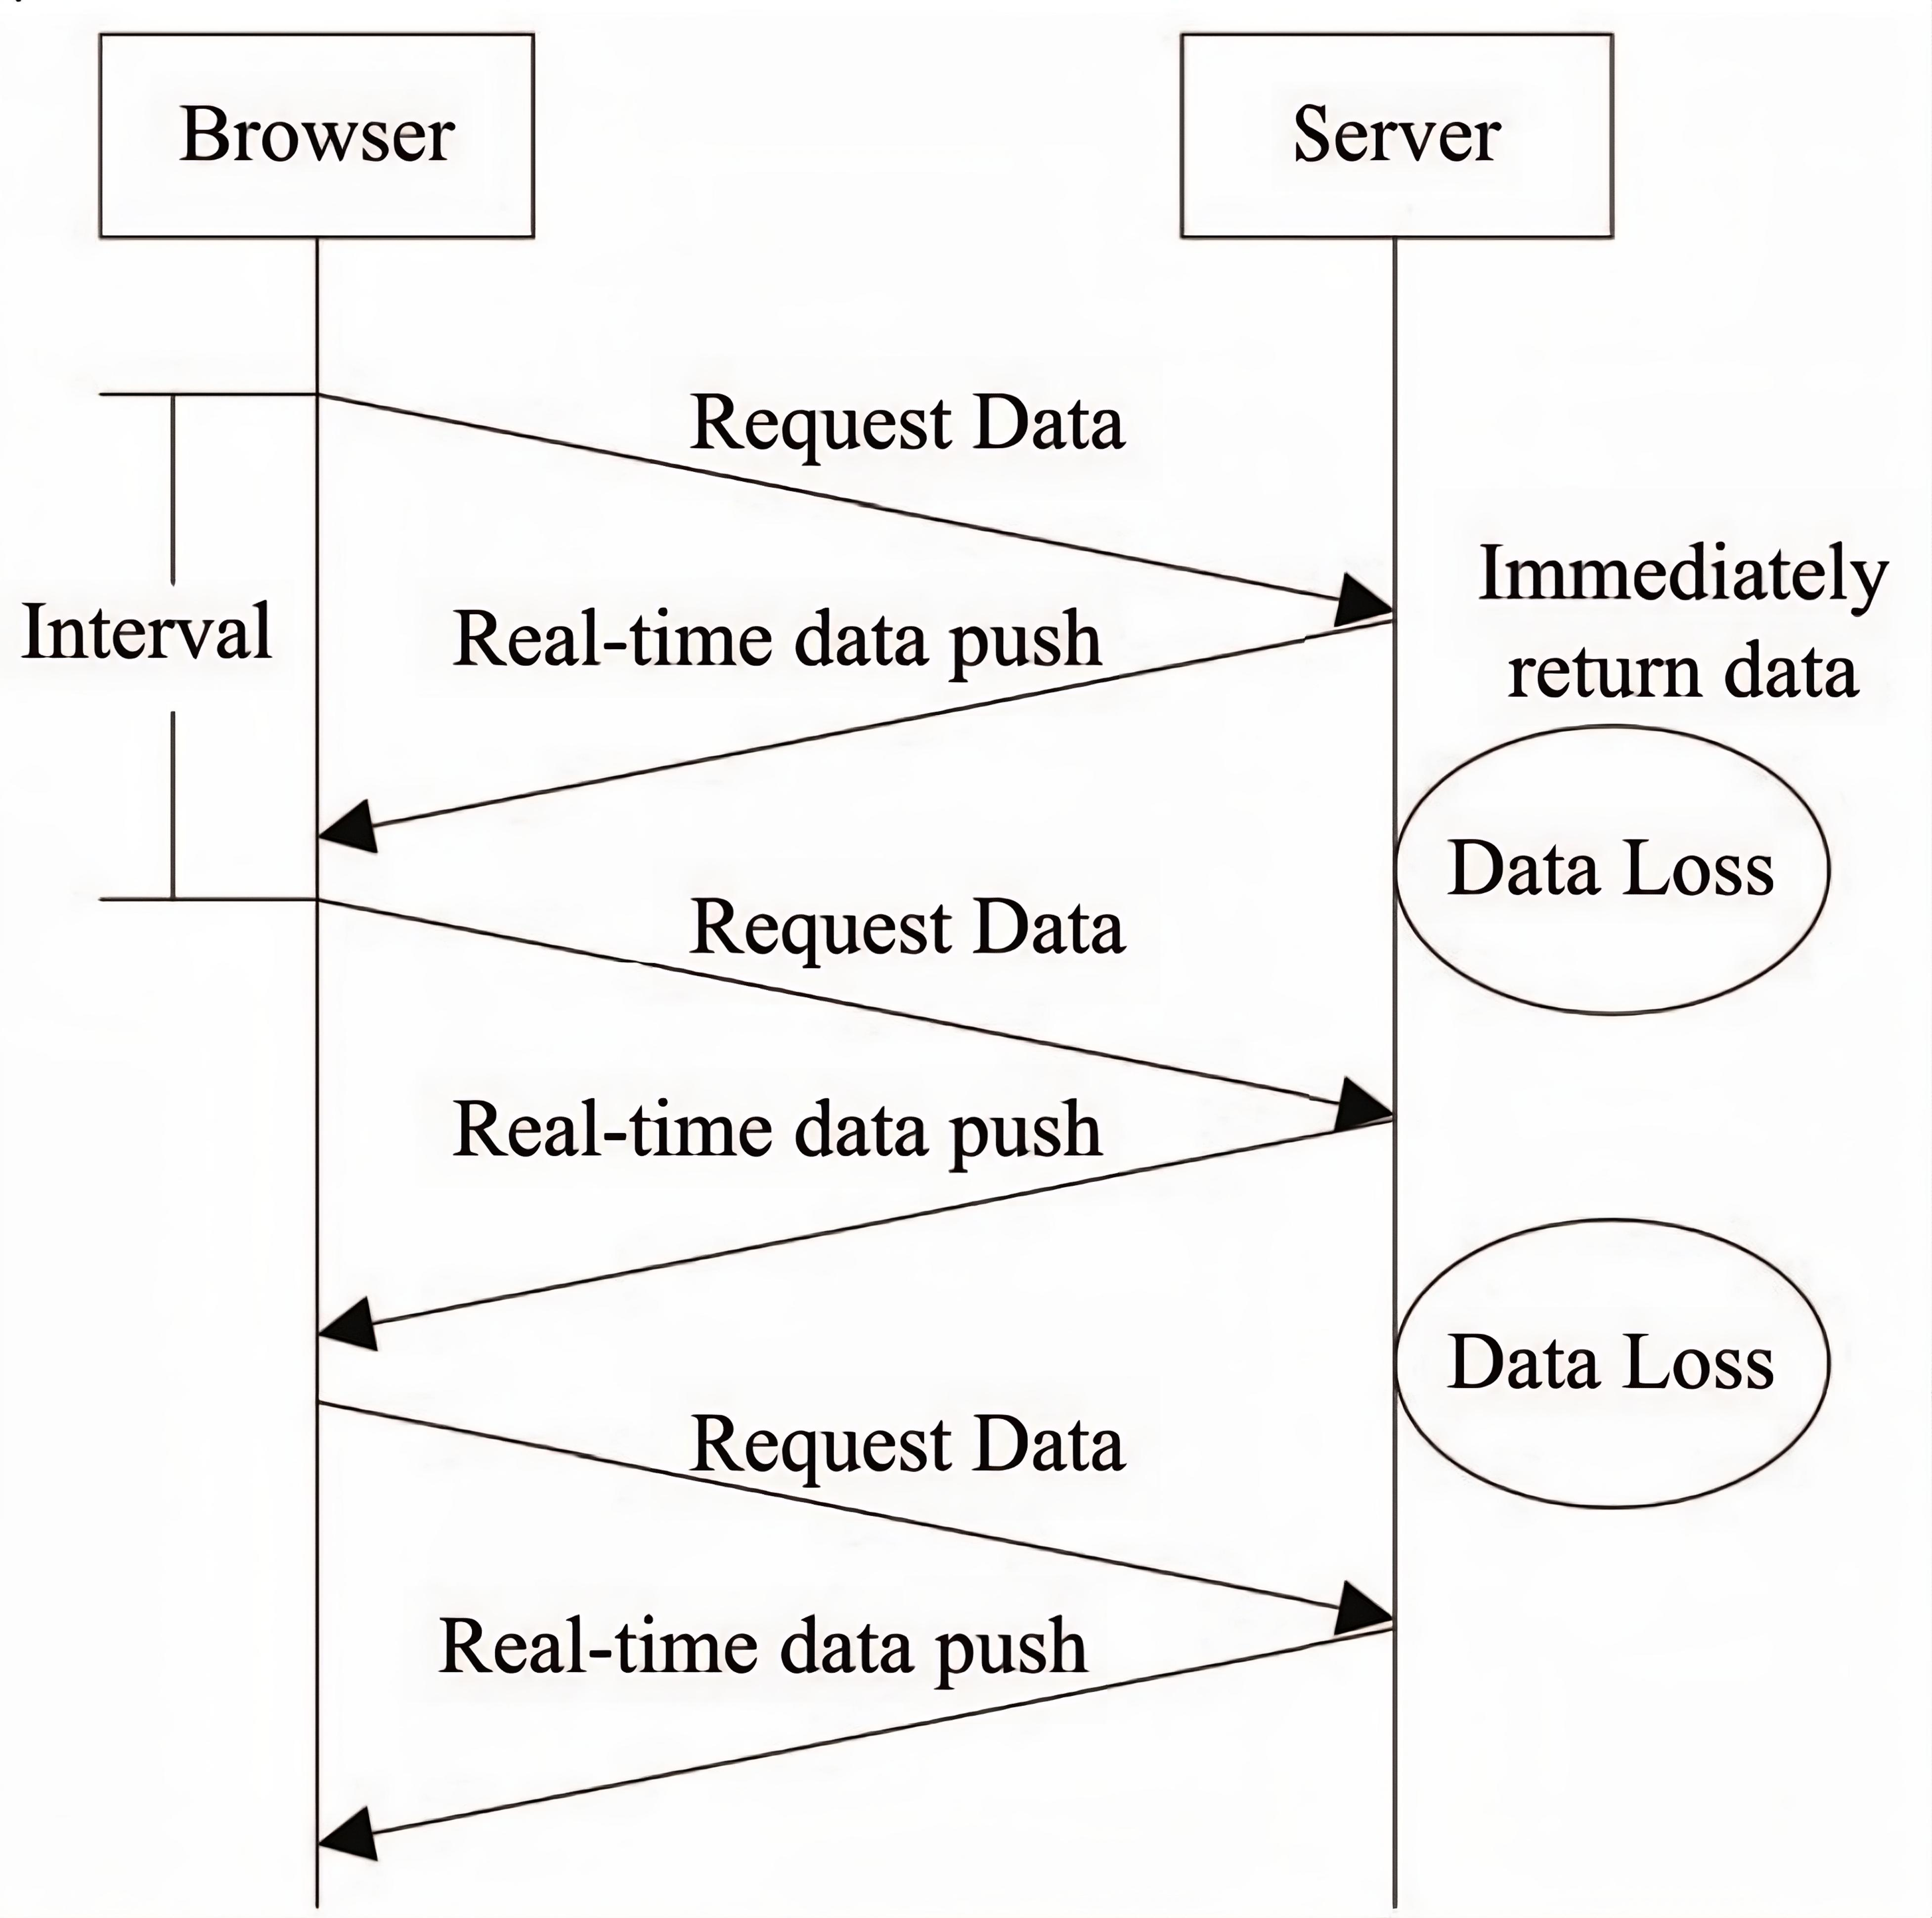
\includegraphics[width=0.7\textwidth]{images/polling.jpeg}
            \end{figure}
        \end{column}
        \begin{column}<+->{0.35\textwidth}
            \begin{itemize}[<+->]
                \item How often to query?
                \item Continuously \alert{short interval} requests will be \alert{washed away} the
                      server. \note{A client can send data and ask for data at the same time. But, if
                          client has no data and server has no data, a request and response will still be
                          generated with all the HTTP headers and thus wasting resources.}
                \item \alert{Long interval} will require more time to reach the client, \alert{no real-time} data.
                      \note{No real-time data because while the client waits, an event could occur and the client will know about it only when the timeout expires.}
            \end{itemize}
        \end{column}
    \end{columns}
\end{frame}

\subsection{HTTP long polling}
\begin{frame}
    \frametitle{HTTP long polling}
    When a client sends a data request, the server will block the request until there is data transfer or timeout before returning.
    \begin{columns}
        \begin{column}{0.7\textwidth}
            \begin{figure}
                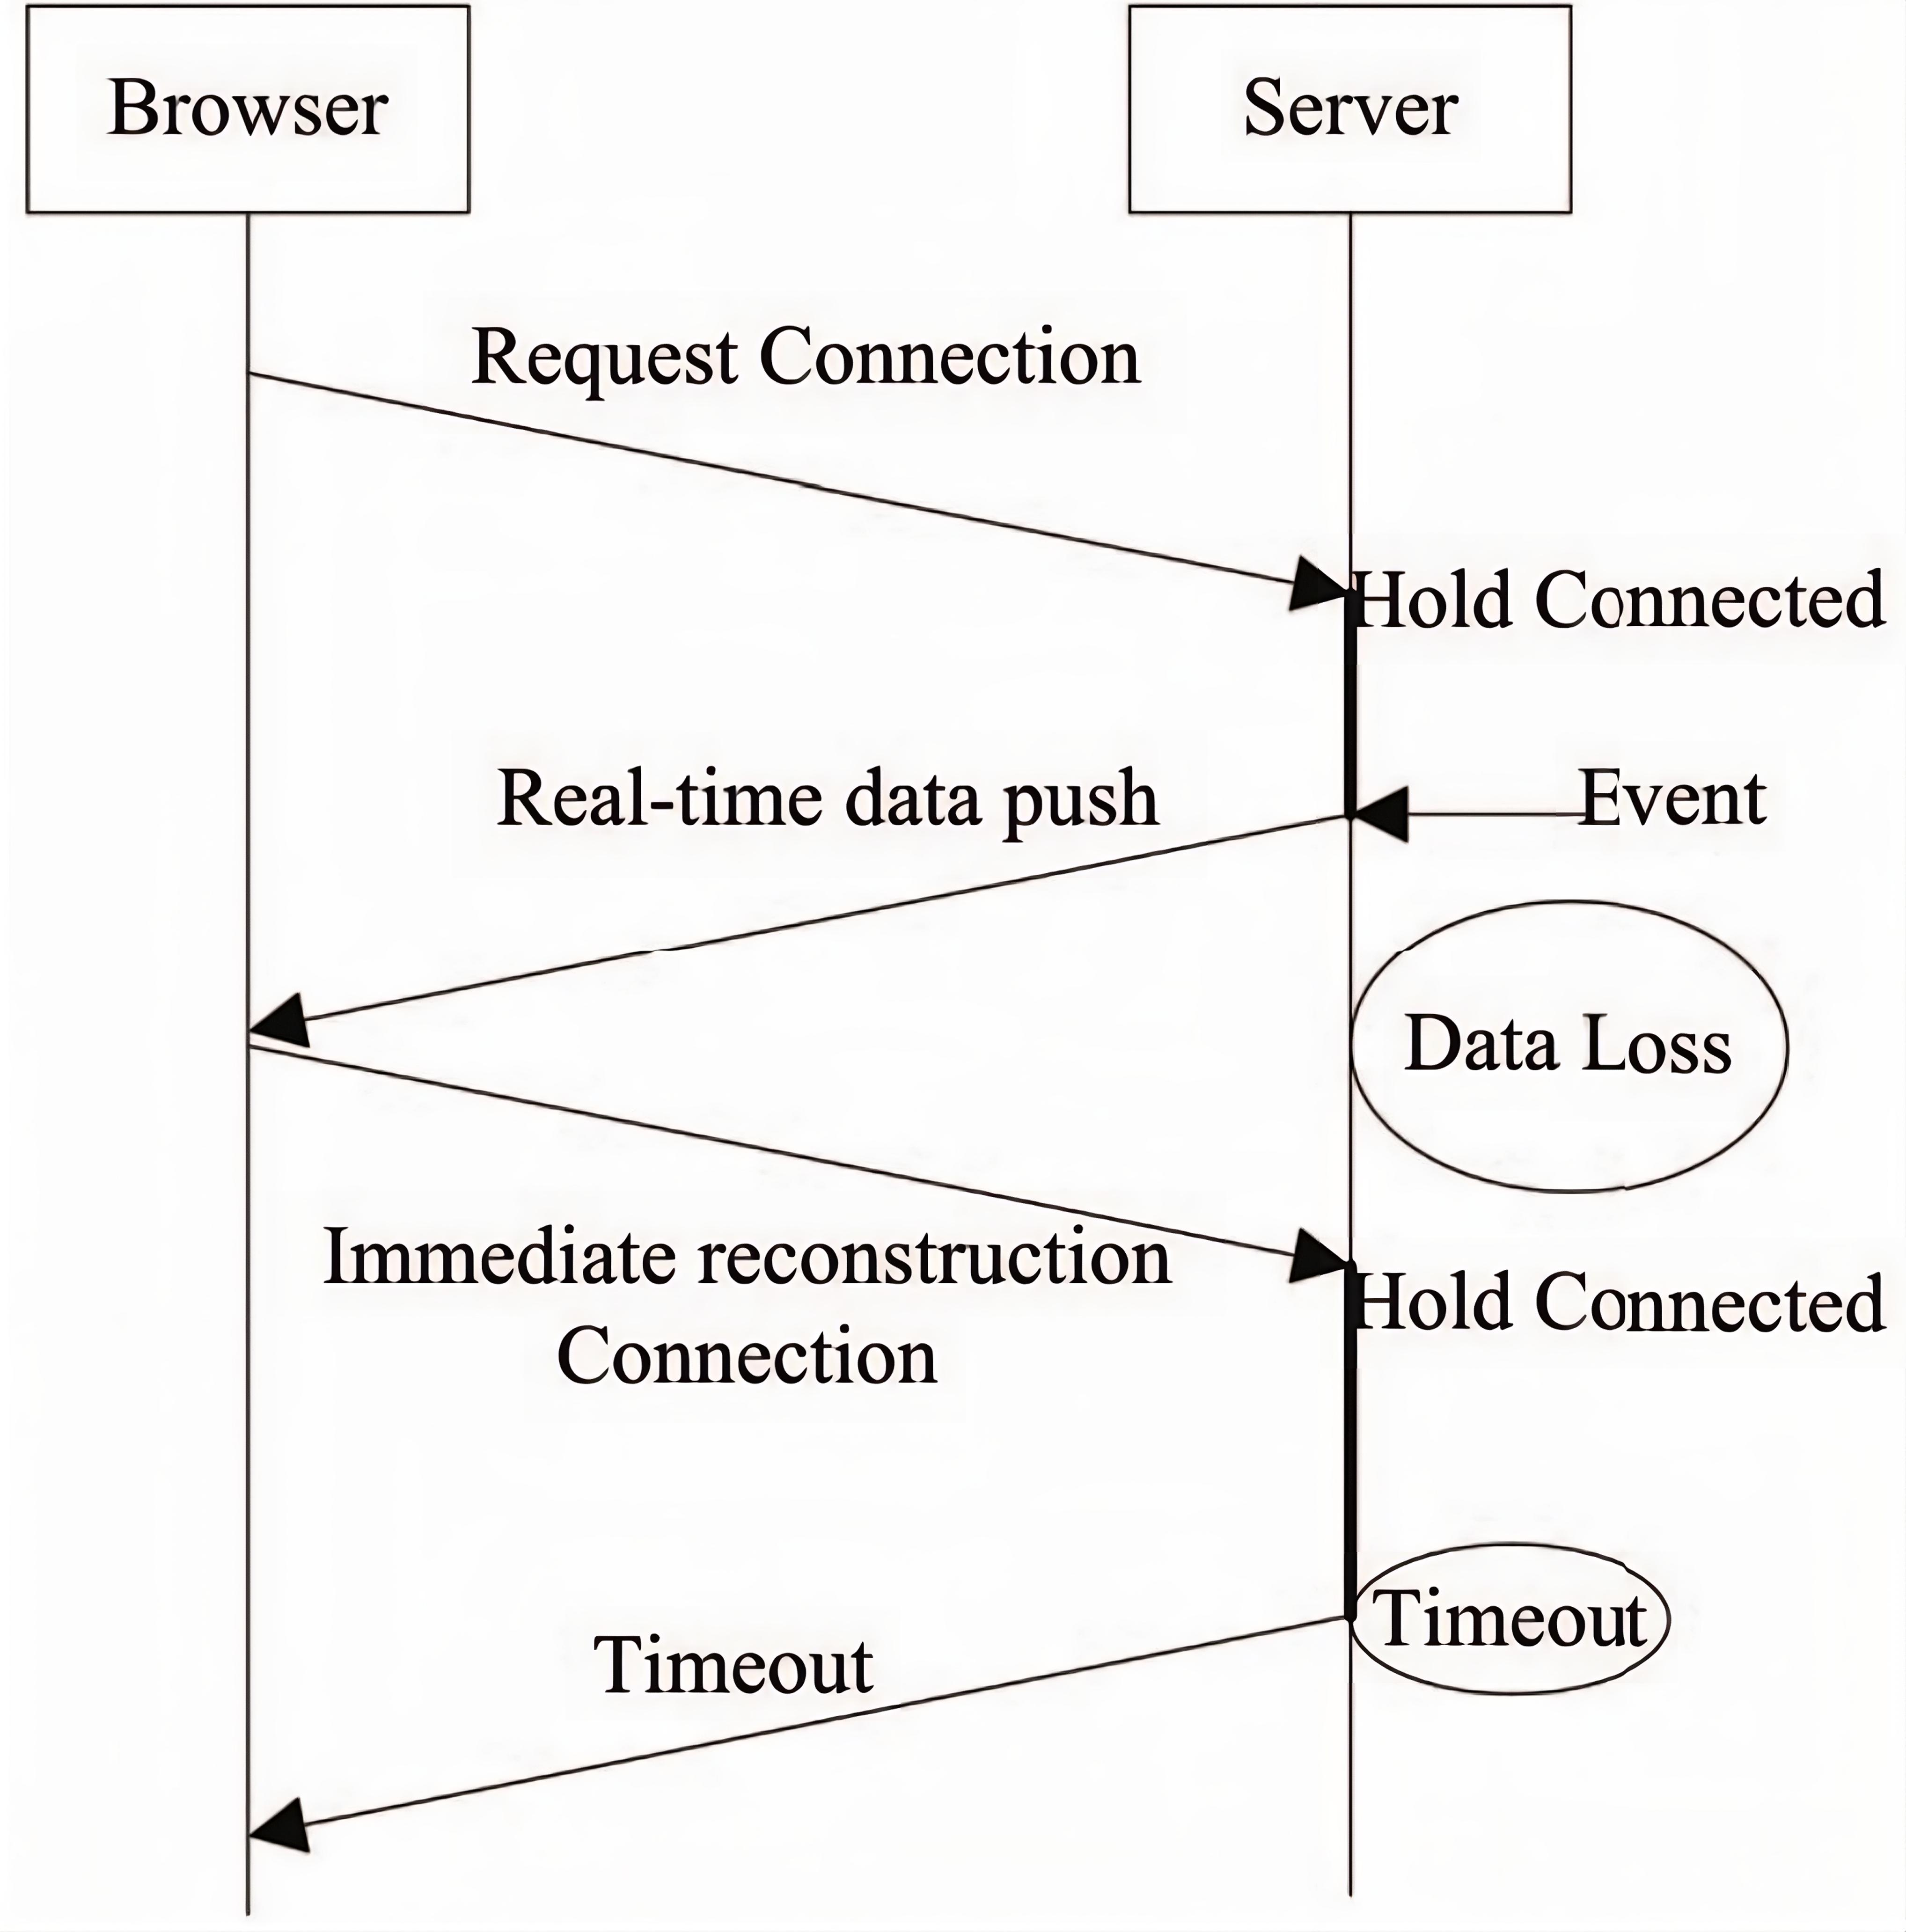
\includegraphics[width=0.7\textwidth]{images/long_polling.jpeg}
            \end{figure}
            \note{Can hold the connection up to a certain time, after that a timeout is exceeded and need a new connection.}
        \end{column}
        \begin{column}<+->{0.35\textwidth}
            \begin{itemize}[<+->]
                \item {\color{green} Solve the short polling frequency to access the server.}
                \item \alert{No bidirectional communication}, server push data.
                      \note{No bidirectional because the client may only send data the first time, but then it will only receive until a timeout and another request is made.}
                      \note{In the normal polling we could have bidirectional because the interval was shorter.}
            \end{itemize}
        \end{column}
    \end{columns}
\end{frame}

\subsection{Streaming}
\begin{frame}
    \frametitle{Streaming}
    Iframe embed a hidden frame in an HTML page, then set it as a long connection request, thus the server can send data to the clients constantly.
    \note{iframe is a html page inside another.}
    \begin{columns}
        \begin{column}{0.7\textwidth}
            \begin{figure}
                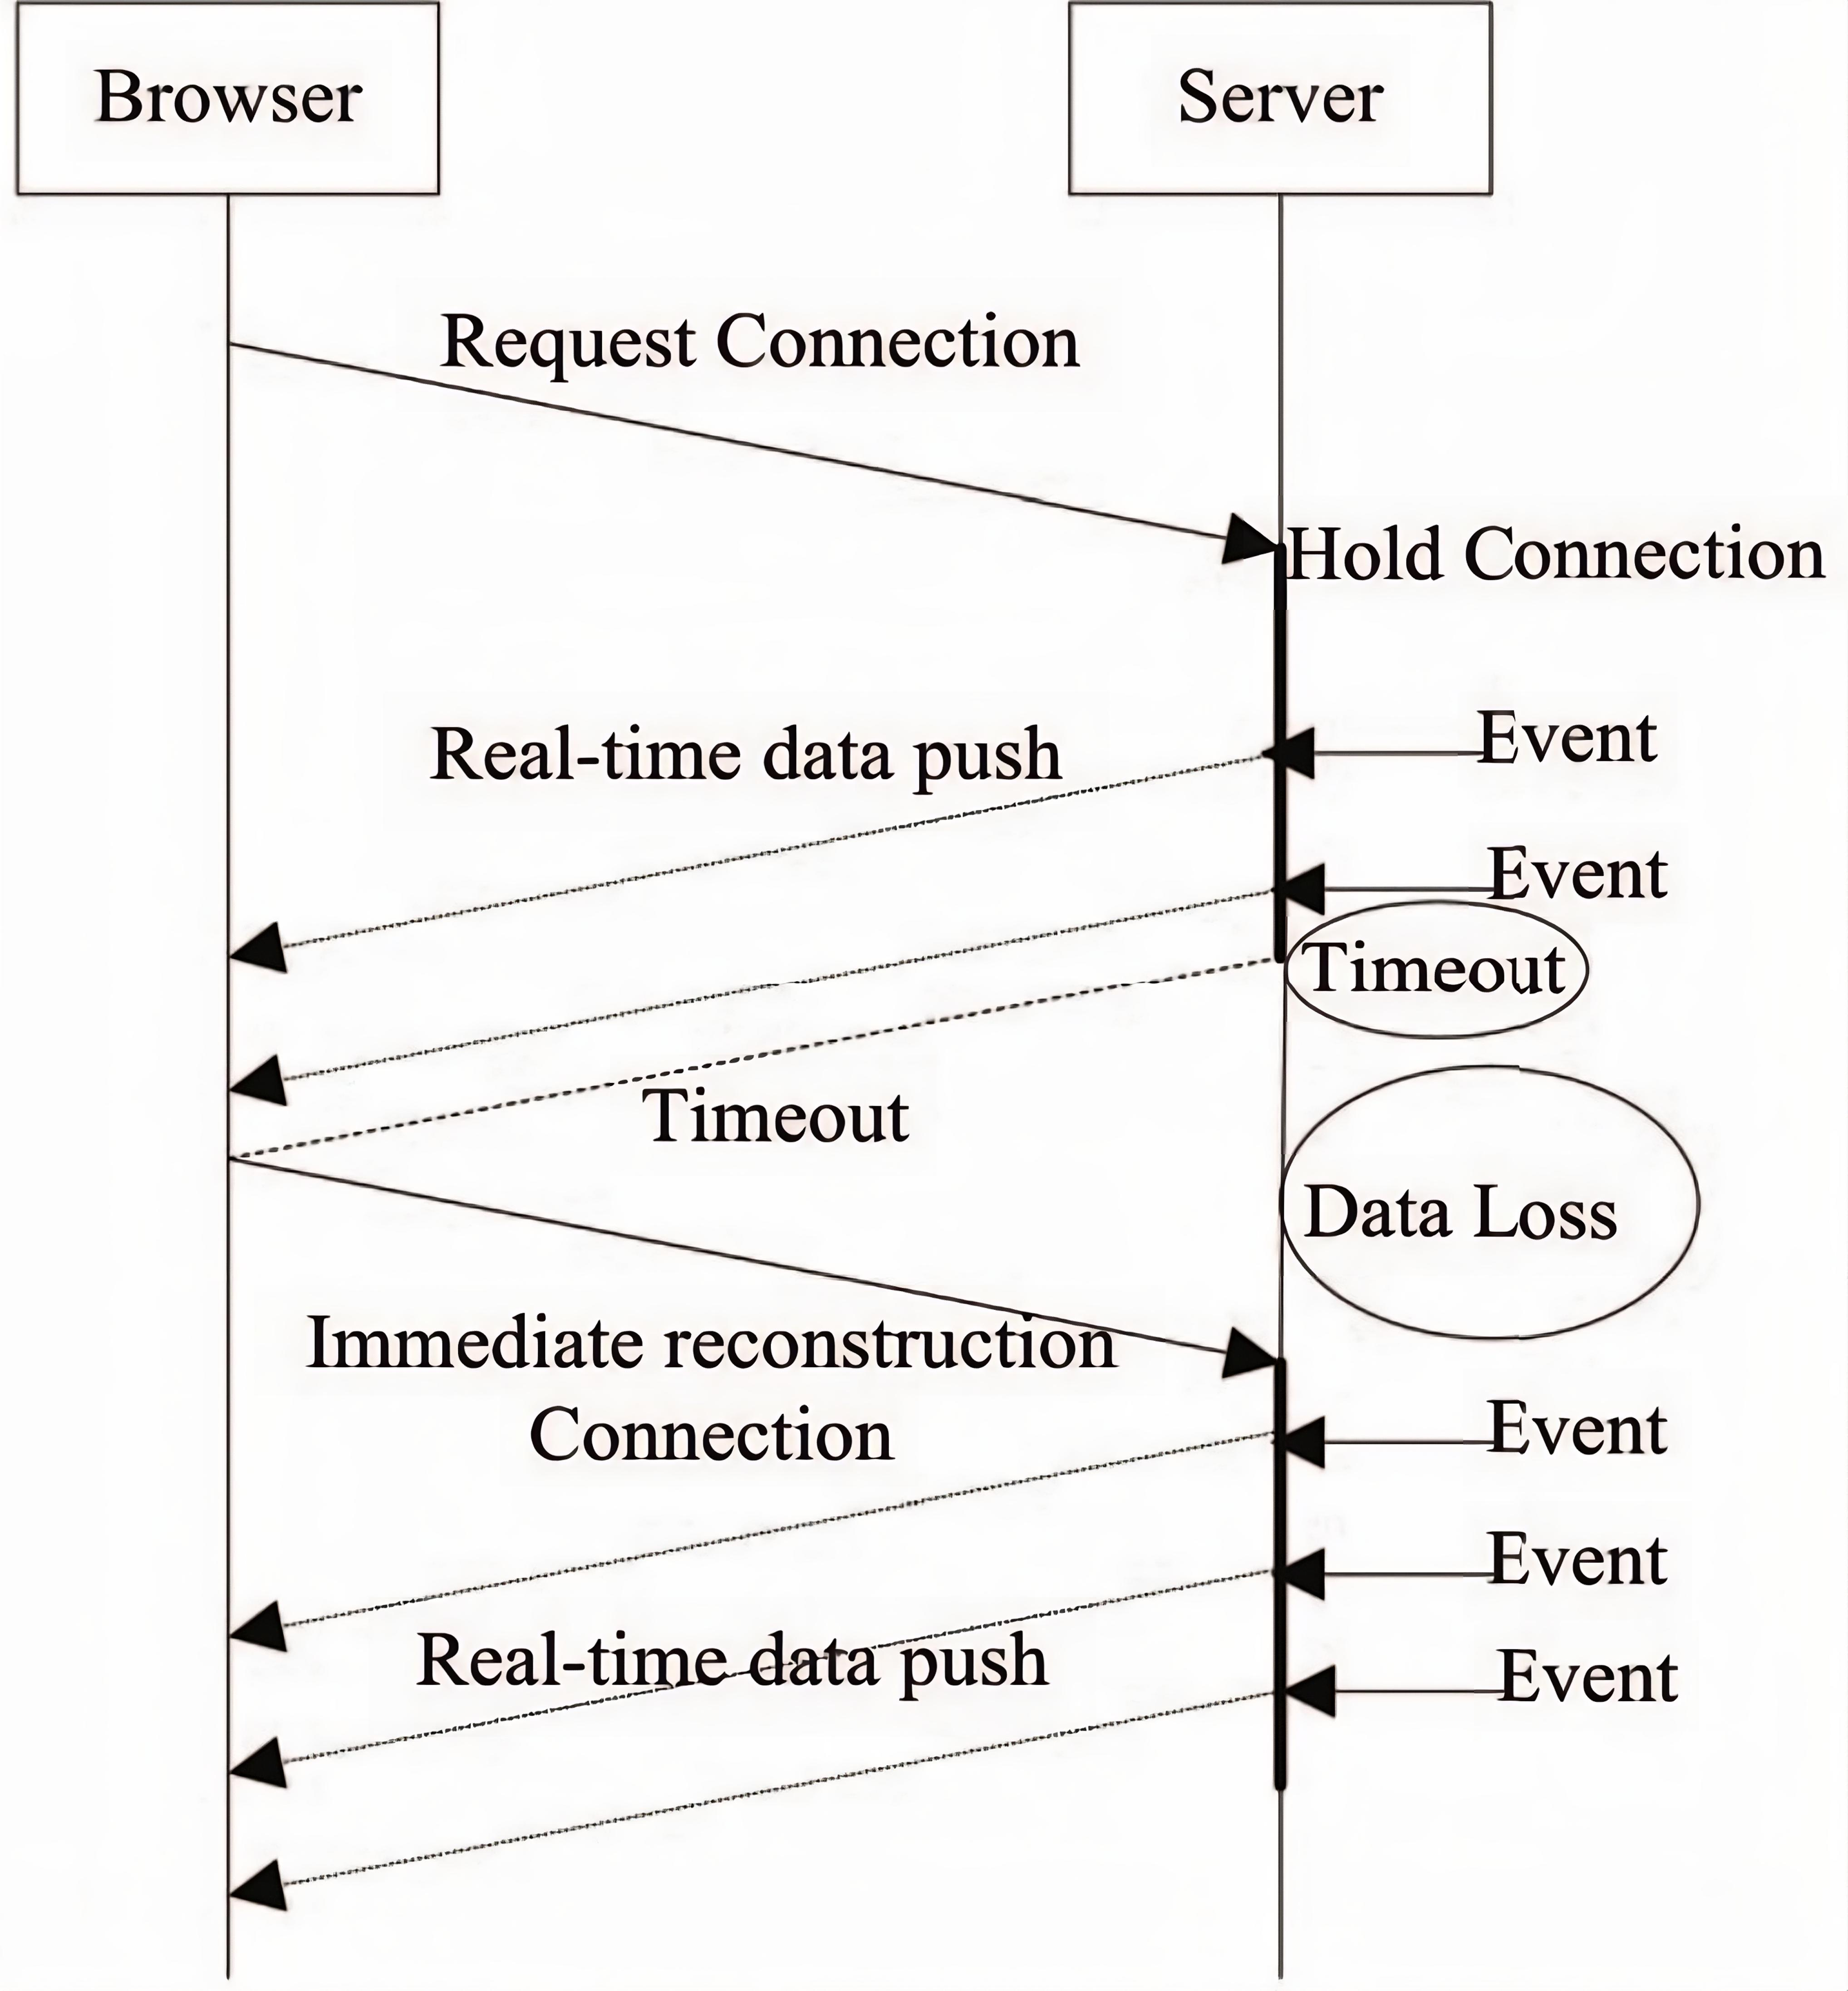
\includegraphics[width=0.7\textwidth]{images/streaming.jpeg}
            \end{figure}
        \end{column}
        \begin{column}<+->{0.35\textwidth}
            \begin{itemize}[<+->]
                \item It can send {\color{green} multiple events} from a {\color{green} single
                              request}.
                \item But, it increases the \alert{burden on the server}, causing the server
                      \alert{performance degradation}, or even collapse. \note{Because the server
                          need to keep the connections alive.}
                \item \alert{No bidirectional communication}.
            \end{itemize}
        \end{column}
    \end{columns}
\end{frame}

\section{WebSocket protocol}

\subsection{Definition}
\begin{frame}
    \frametitle{RFC 6455}
    \framesubtitle{Keywords}
    \begin{itemize}[<+->]
        \item The WebSocket Protocol enables \alert<+->{two-way communication} between a
              \alert<+->{client} running untrusted code in a controlled environment to a
              \alert<+->{remote host} that has \alert<+->{opted-in} to communications from
              that code. \note{opted-in is important because with polling any HTTP server
                  would accept it, but here additional steps are needed.}
        \item The protocol consists of an opening \alert<+->{handshake} followed by basic
              \alert<+->{message framing}, layered over \alert<+->{TCP}. \note{Handshake
                  means client and server have to agree that they can both use the protocol and
                  the server has to prove it.} \note{Message framing because we do not want to
                  send every time the headers.} \note{TCP means it is reliable, no messages will
                  be lost.}
        \item The goal of this technology is to provide a mechanism for
              \alert<+->{browser-based} applications that need two-way communication with
              servers.
    \end{itemize}
\end{frame}

\begin{frame}
    \frametitle{WebSocket}
    \begin{figure}
        \includegraphics[width=0.8\textwidth]{images/WebSocket.jpeg}
    \end{figure}
    \note{There is the initial handshake, after that, client and server can send and receive data at any moment without further interaction.}
    \note{There is no timeout. If it disconnects, it is because of an error and to establish the connection, the handshake has to be done again.}
\end{frame}

\subsection{Handshake}
\begin{frame}
    \frametitle{Handshake}
    \begin{itemize}[<+->]
        \item For WebSocket-based communication, a \alert{WebSocket session} should be
              established first.
        \item To establish a session, client sends a WebSocket \alert{Upgrade Request} to the
              server, upon which server responds with a WebSocket \alert{Upgrade Response}.
              \note{With the Upgrade Response, the server proves that it can communicate with
                  WebSockets.}
        \item From this point forward, the client and server can \alert{send data back and
                  forth in asynchronous full-duplex mode}.
    \end{itemize}
\end{frame}

\subsubsection{Upgrade Request}
\begin{frame}
    \frametitle{WebSocket Upgrade Request}
    \begin{columns}
        \begin{column}{0.6\textwidth}
            \texttt{\alert<2>{GET} \alert<3>{/chat} \alert<2>{HTTP/1.1}\\
                Host: server.example.com\\
                \alert<4>{Upgrade: WebSocket}\\
                \alert<4>{Connection: Upgrade}\\
                \alert<5>{Sec-WebSocket-Key: dGhlIHNhbXBsZSBub25jZQ==}\\
                Origin: http://example.com\\
                \alert<6>{Sec-WebSocket-Protocol: chat, superchat}\\
                \alert<7>{Sec-WebSocket-Version: 13}
            }
        \end{column}
        \begin{column}<+->{0.45\textwidth}
            \begin{itemize}
                \item<2-| alert@2> HTTP GET request.
                \item<3-| alert@3> URI to identify endpoint.
                      \note{Different URI can be used to identify different endpoints. A URI can be regular HTTP, another can be WebSocket.}
                \item<4-| alert@4> Headers indicating the will to switch from regular HTTP to WebSocket.
                \item<5-| alert@5> A key the server has to use to prove that it can use WebSockets.
                \item<6-| alert@6> WebSocket protocols.
                \item<7-| alert@7> WebSocket version.
            \end{itemize}
        \end{column}
    \end{columns}
\end{frame}

\subsubsection{Upgrade Response}
\begin{frame}
    \frametitle{WebSocket Upgrade Response}
    \begin{columns}
        \begin{column}{0.6\textwidth}
            \texttt{HTTP/1.1 \alert<2>{101 Switching protocols}\\
                \alert<2>{Upgrade: WebSocket}\\
                \alert<2>{Connection: Upgrade}\\
                \alert<3>{Sec-WebSocket-Accept: dGhlIHNhbXBsZSBub25jZQ==}\\
                Origin: http://example.com\\
                \alert<4>{Sec-WebSocket-Protocol: chat}
            }
        \end{column}
        \begin{column}<+->{0.45\textwidth}
            \begin{itemize}
                \item<2-| alert@2> Server confirms it supports WebSocket.
                \item<3-| alert@3> Server proves that it can use WebSocket. Client checks it.
                      \note{There is a specific algorithm to generate this Header from a key.}
                \item<4-| alert@4> Server tells which protocol it supports.
            \end{itemize}
        \end{column}
    \end{columns}
\end{frame}

\subsection{Frame}
\begin{frame}
    \frametitle{WebSocket Frame}
    \begin{itemize}[<+->]
        \item After the handshake is successful, client and server can \alert{communicate in
                  full-duplex} by using frames.
        \item The added \alert{overhead} to the payload data is \alert{minimal} because it
              does not send all the HTTP headers for each frame.
        \item Each frame adds \alert{at least 2 bytes of overhead} to the payload data.
              Depending on the length of the payload data and the direction of the
              communication, the length of the overhead \alert{may increase up to 14 bytes}.
    \end{itemize}
\end{frame}

\begin{frame}
    \frametitle{WebSocket Frame Structure}
    \note{We will not go into the details because it is out of the scope of this presentation and, as mentioned earlier, the added overhead to the payload data is minimal.}
    \begin{figure}
        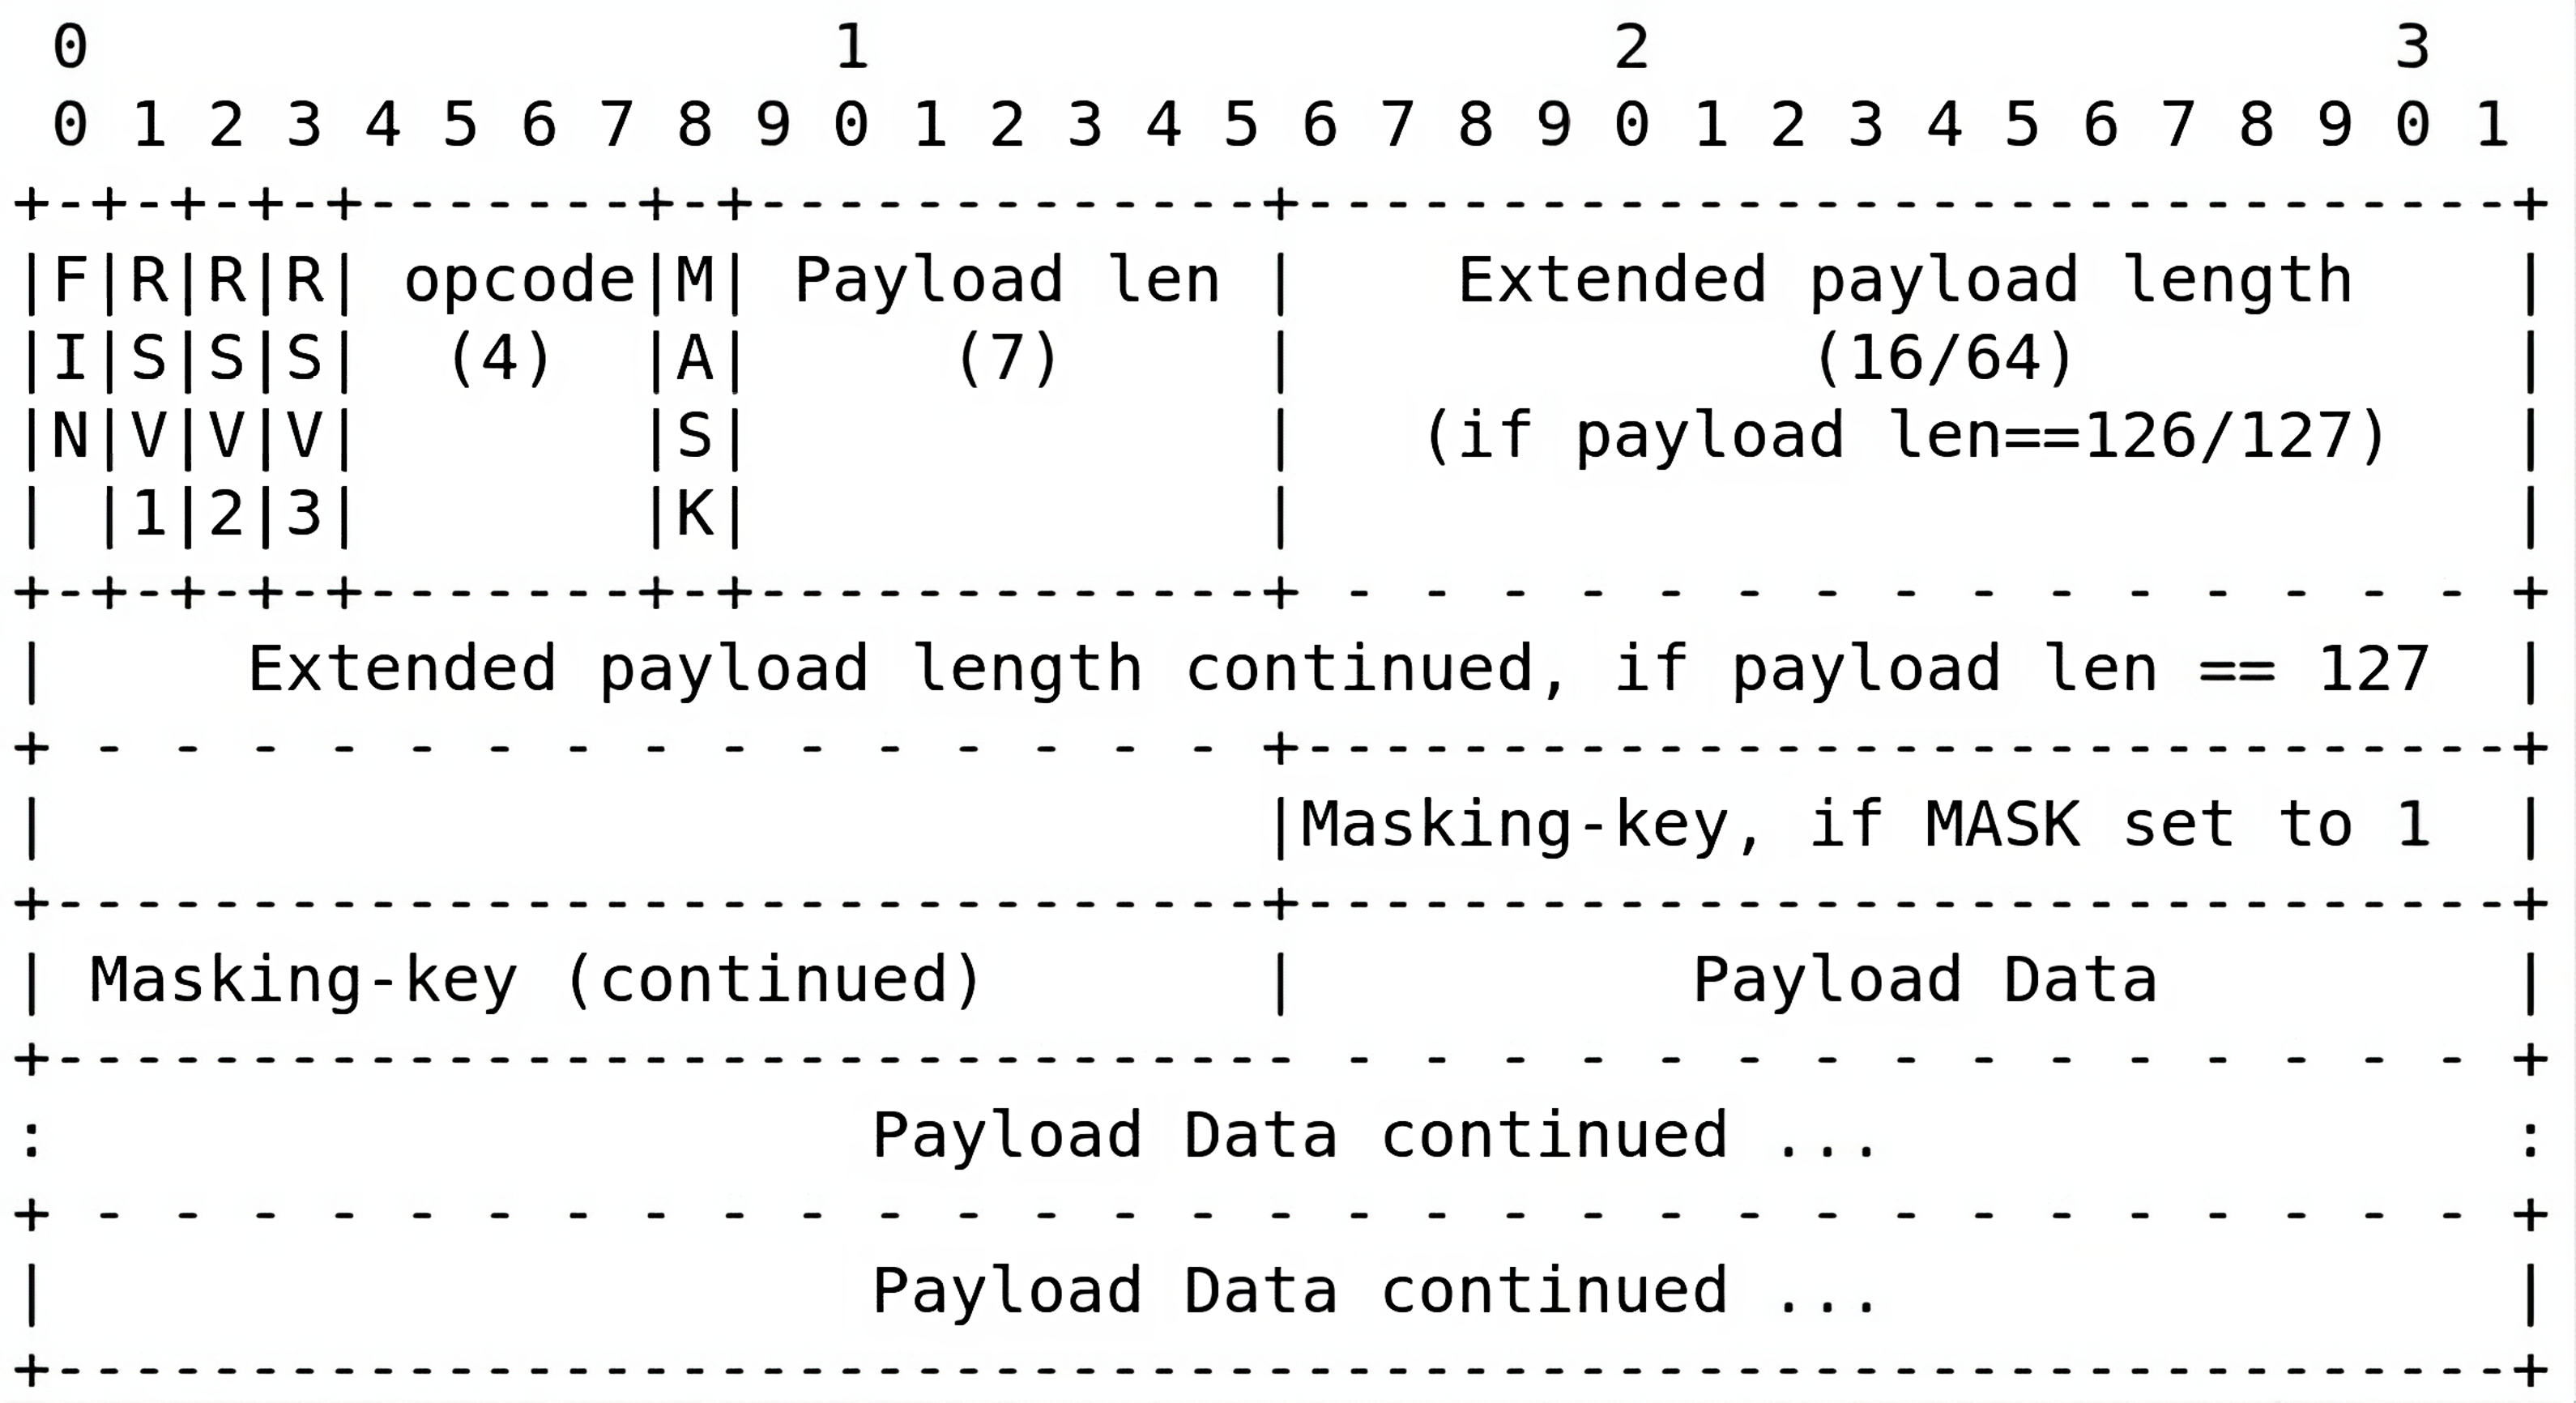
\includegraphics[width=1\textwidth]{images/message_frame.png}
    \end{figure}
\end{frame}

\subsection{API}
\begin{frame}
    \frametitle{WebSocket API}
    The API is defined by its states of readiness, responses to a networking or messaging \alert{event}.
    \begin{table}
        \centering
        \begin{tabular}{|c | p{0.6\linewidth}|}
            \hline
            \textbf{Callback}  & \textbf{Description}                                                                                                    \\
            \hline
            \hline
            \texttt{onopen}    & invoked when WebSocket \texttt{session is established}, signalizes that the protocol is ready to transfer payload data \\
            \hline
            \texttt{onerror}   & invoked whenever an \texttt{error occurs}                                                                              \\
            \hline
            \texttt{onclose}   & invoked when one of the peers has \texttt{terminated the session}                                                      \\
            \hline
            \texttt{onmessage} & invoked when an \texttt{incoming message} from another peer has arrived                                                \\
            \hline
        \end{tabular}
    \end{table}
\end{frame}

\begin{frame}
    \nocite{*}
    \frametitle{References}
    \bibliographystyle{amsalpha}
    \bibliography{bib.bib}
\end{frame}
\end{document}